%
% 6.006 problem set 4 solutions template
%
\documentclass[12pt,twoside]{article}

\usepackage{amsmath}
\usepackage{color}
\usepackage{listings}
\usepackage{graphicx}

% Cross-references for handout numbers.

% Updated to include SMA course for Fall 2001 -- cel

\newcommand{\name}{}


\usepackage{latexsym}
%\usepackage{bbm}
\usepackage{times,url}
\usepackage{clrscode}

\newcommand{\mitst}[1]{\begin{description}
\item[MIT students:] #1
\end{description}}
\newcommand{\smast}[1]{\begin{description}
\item[SMA students:] #1
\end{description}}

\newcommand{\profs}{Professors Srini Devadas, Nancy Lynch and Vinod Vaikuntanathan}
\newcommand{\subj}{6.006}

\newlength{\toppush}
\setlength{\toppush}{2\headheight}
\addtolength{\toppush}{\headsep}

\newcommand{\htitle}[2]{\noindent\vspace*{-\toppush}\newline\parbox{6.5in}
{\textit{Introduction to Algorithms: 6.006}\hfill\name\newline
Massachusetts Institute of Technology \hfill #2\newline
\profs\hfill #1 \vspace*{-.5ex}\newline
\mbox{}\hrulefill\mbox{}}\vspace*{1ex}\mbox{}\newline
\begin{center}{\Large\bf #1}\end{center}}

\newcommand{\handout}[2]{\thispagestyle{empty}
 \markboth{#1}{#1}
 \pagestyle{myheadings}\htitle{#1}{#2}}

\newcommand{\htitlewithouttitle}[2]{\noindent\vspace*{-\toppush}\newline\parbox{6.5in}
{\textit{Introduction to Algorithms}\hfill#2\newline
Massachusetts Institute of Technology \hfill 6.006\newline
%Singapore-MIT Alliance \hfill SMA5503\newline
\profs\hfill Handout #1\vspace*{-.5ex}\newline
\mbox{}\hrulefill\mbox{}}\vspace*{1ex}\mbox{}\newline}

\newcommand{\handoutwithouttitle}[2]{\thispagestyle{empty}
 \markboth{Handout \protect\ref{#1}}{Handout \protect\ref{#1}}
 \pagestyle{myheadings}\htitlewithouttitle{\protect\ref{#1}}{#2}}

\newcommand{\exam}[2]{% parameters: exam name, date
 \thispagestyle{empty}
 \markboth{\subj\ #1\hspace{1in}Name\hrulefill\ \ }%
          {\subj\ #1\hspace{1in}Name\hrulefill\ \ }
 \pagestyle{myheadings}\examtitle{#1}{#2}
 \renewcommand{\theproblem}{Problem \arabic{problemnum}}
}
\newcommand{\examsolutions}[3]{% parameters: handout, exam name, date
 \thispagestyle{empty}
 \markboth{Handout \protect\ref{#1}: #2}{Handout \protect\ref{#1}: #2}
% \pagestyle{myheadings}\htitle{\protect\ref{#1}}{#2}{#3}
 \pagestyle{myheadings}\examsolutionstitle{\protect\ref{#1}} {#2}{#3}
 \renewcommand{\theproblem}{Problem \arabic{problemnum}}
}
\newcommand{\examsolutionstitle}[3]{\noindent\vspace*{-\toppush}\newline\parbox{6.5in}
{\textit{Introduction to Algorithms}\hfill#3\newline
Massachusetts Institute of Technology \hfill 6.006\newline
%Singapore-MIT Alliance \hfill SMA5503\newline
\profs\hfill Handout #1\vspace*{-.5ex}\newline
\mbox{}\hrulefill\mbox{}}\vspace*{1ex}\mbox{}\newline
\begin{center}{\Large\bf #2}\end{center}}

\newcommand{\takehomeexam}[2]{% parameters: exam name, date
 \thispagestyle{empty}
 \markboth{\subj\ #1\hfill}{\subj\ #1\hfill}
 \pagestyle{myheadings}\examtitle{#1}{#2}
 \renewcommand{\theproblem}{Problem \arabic{problemnum}}
}

\makeatletter
\newcommand{\exambooklet}[2]{% parameters: exam name, date
 \thispagestyle{empty}
 \markboth{\subj\ #1}{\subj\ #1}
 \pagestyle{myheadings}\examtitle{#1}{#2}
 \renewcommand{\theproblem}{Problem \arabic{problemnum}}
 \renewcommand{\problem}{\newpage
 \item \let\@currentlabel=\theproblem
 \markboth{\subj\ #1, \theproblem}{\subj\ #1, \theproblem}}
}
\makeatother


\newcommand{\examtitle}[2]{\noindent\vspace*{-\toppush}\newline\parbox{6.5in}
{\textit{Introduction to Algorithms}\hfill#2\newline
Massachusetts Institute of Technology \hfill 6.006 Spring 2014\newline
%Singapore-MIT Alliance \hfill SMA5503\newline
\profs\hfill #1\vspace*{-.5ex}\newline
\mbox{}\hrulefill\mbox{}}\vspace*{1ex}\mbox{}\newline
\begin{center}{\Large\bf #1}\end{center}}

\newcommand{\grader}[1]{\hspace{1cm}\textsf{\textbf{#1}}\hspace{1cm}}

\newcommand{\points}[1]{[#1 points]\ }
\newcommand{\parts}[1]
{
  \ifnum#1=1
  (1 part)
  \else
  (#1 parts)
  \fi
  \ 
}

\newcommand{\bparts}{\begin{problemparts}}
\newcommand{\eparts}{\end{problemparts}}
\newcommand{\ppart}{\problempart}

%\newcommand{\lg} {lg\ }

\setlength{\oddsidemargin}{0pt}
\setlength{\evensidemargin}{0pt}
\setlength{\textwidth}{6.5in}
\setlength{\topmargin}{0in}
\setlength{\textheight}{8.5in}


\newcommand{\Spawn}{{\bf spawn} }
\newcommand{\Sync}{{\bf sync}}

\renewcommand{\cases}[1]{\left\{ \begin{array}{ll}#1\end{array}\right.}
\newcommand{\cif}[1]{\mbox{if $#1$}}
\newcommand{\cwhen}[1]{\mbox{when $#1$}}

\newcounter{problemnum}
\newcommand{\theproblem}{Problem \theproblemsetnum-\arabic{problemnum}}
\newenvironment{problems}{
        \begin{list}{{\bf \theproblem. \hspace*{0.5em}}}
        {\setlength{\leftmargin}{0em}
         \setlength{\rightmargin}{0em}
         \setlength{\labelwidth}{0em}
         \setlength{\labelsep}{0em}
         \usecounter{problemnum}}}{\end{list}}
\makeatletter
\newcommand{\problem}[1][{}]{\item \let\@currentlabel=\theproblem \textbf{#1}}
\makeatother

\newcounter{problempartnum}[problemnum]
\newenvironment{problemparts}{
        \begin{list}{{\bf (\alph{problempartnum})}}
        {\setlength{\leftmargin}{2.5em}
         \setlength{\rightmargin}{2.5em}
         \setlength{\labelsep}{0.5em}}}{\end{list}}
\newcommand{\problempart}{\addtocounter{problempartnum}{1}\item}

\newenvironment{truefalseproblemparts}{
        \begin{list}{{\bf (\alph{problempartnum})\ \ \ T\ \ F\hfil}}
        {\setlength{\leftmargin}{4.5em}
         \setlength{\rightmargin}{2.5em}
         \setlength{\labelsep}{0.5em}
         \setlength{\labelwidth}{4.5em}}}{\end{list}}

\newcounter{exercisenum}
\newcommand{\theexercise}{Exercise \theproblemsetnum-\arabic{exercisenum}}
\newenvironment{exercises}{
        \begin{list}{{\bf \theexercise. \hspace*{0.5em}}}
        {\setlength{\leftmargin}{0em}
         \setlength{\rightmargin}{0em}
         \setlength{\labelwidth}{0em}
         \setlength{\labelsep}{0em}
        \usecounter{exercisenum}}}{\end{list}}
\makeatletter
\newcommand{\exercise}{\item \let\@currentlabel=\theexercise}
\makeatother

\newcounter{exercisepartnum}[exercisenum]
%\newcommand{\problem}[1]{\medskip\mbox{}\newline\noindent{\bf Problem #1.}\hspace*{1em}}
%\newcommand{\exercise}[1]{\medskip\mbox{}\newline\noindent{\bf Exercise #1.}\hspace*{1em}}

\newenvironment{exerciseparts}{
        \begin{list}{{\bf (\alph{exercisepartnum})}}
        {\setlength{\leftmargin}{2.5em}
         \setlength{\rightmargin}{2.5em}
         \setlength{\labelsep}{0.5em}}}{\end{list}}
\newcommand{\exercisepart}{\addtocounter{exercisepartnum}{1}\item}


% Macros to make captions print with small type and 'Figure xx' in bold.
\makeatletter
\def\fnum@figure{{\bf Figure \thefigure}}
\def\fnum@table{{\bf Table \thetable}}
\let\@mycaption\caption
%\long\def\@mycaption#1[#2]#3{\addcontentsline{\csname
%  ext@#1\endcsname}{#1}{\protect\numberline{\csname 
%  the#1\endcsname}{\ignorespaces #2}}\par
%  \begingroup
%    \@parboxrestore
%    \small
%    \@makecaption{\csname fnum@#1\endcsname}{\ignorespaces #3}\par
%  \endgroup}
%\def\mycaption{\refstepcounter\@captype \@dblarg{\@mycaption\@captype}}
%\makeatother
\let\mycaption\caption
%\newcommand{\figcaption}[1]{\mycaption[]{#1}}

\newcounter{totalcaptions}
\newcounter{totalart}

\newcommand{\figcaption}[1]{\addtocounter{totalcaptions}{1}\caption[]{#1}}

% \psfigures determines what to do for figures:
%       0 means just leave vertical space
%       1 means put a vertical rule and the figure name
%       2 means insert the PostScript version of the figure
%       3 means put the figure name flush left or right
\newcommand{\psfigures}{0}
\newcommand{\spacefigures}{\renewcommand{\psfigures}{0}}
\newcommand{\rulefigures}{\renewcommand{\psfigures}{1}}
\newcommand{\macfigures}{\renewcommand{\psfigures}{2}}
\newcommand{\namefigures}{\renewcommand{\psfigures}{3}}

\newcommand{\figpart}[1]{{\bf (#1)}\nolinebreak[2]\relax}
\newcommand{\figparts}[2]{{\bf (#1)--(#2)}\nolinebreak[2]\relax}


\macfigures     % STATE

% When calling \figspace, make sure to leave a blank line afterward!!
% \widefigspace is for figures that are more than 28pc wide.
\newlength{\halffigspace} \newlength{\wholefigspace}
\newlength{\figruleheight} \newlength{\figgap}
\newcommand{\setfiglengths}{\ifnum\psfigures=1\setlength{\figruleheight}{\hruleheight}\setlength{\figgap}{1em}\else\setlength{\figruleheight}{0pt}\setlength{\figgap}{0em}\fi}
\newcommand{\figspace}[2]{\ifnum\psfigures=0\leavefigspace{#1}\else%
\setfiglengths%
\setlength{\wholefigspace}{#1}\setlength{\halffigspace}{.5\wholefigspace}%
\rule[-\halffigspace]{\figruleheight}{\wholefigspace}\hspace{\figgap}#2\fi}
\newlength{\widefigspacewidth}
% Make \widefigspace put the figure flush right on the text page.
\newcommand{\widefigspace}[2]{
\ifnum\psfigures=0\leavefigspace{#1}\else%
\setfiglengths%
\setlength{\widefigspacewidth}{28pc}%
\addtolength{\widefigspacewidth}{-\figruleheight}%
\setlength{\wholefigspace}{#1}\setlength{\halffigspace}{.5\wholefigspace}%
\makebox[\widefigspacewidth][r]{#2\hspace{\figgap}}\rule[-\halffigspace]{\figruleheight}{\wholefigspace}\fi}
\newcommand{\leavefigspace}[1]{\setlength{\wholefigspace}{#1}\setlength{\halffigspace}{.5\wholefigspace}\rule[-\halffigspace]{0em}{\wholefigspace}}

% Commands for including figures with macpsfig.
% To use these commands, documentstyle ``macpsfig'' must be specified.
\newlength{\macfigfill}
\makeatother
\newlength{\bbx}
\newlength{\bby}
\newcommand{\macfigure}[5]{\addtocounter{totalart}{1}
\ifnum\psfigures=2%
\setlength{\bbx}{#2}\addtolength{\bbx}{#4}%
\setlength{\bby}{#3}\addtolength{\bby}{#5}%
\begin{flushleft}
\ifdim#4>28pc\setlength{\macfigfill}{#4}\addtolength{\macfigfill}{-28pc}\hspace*{-\macfigfill}\fi%
\mbox{\psfig{figure=./#1.ps,%
bbllx=#2,bblly=#3,bburx=\bbx,bbury=\bby}}
\end{flushleft}%
\else\ifdim#4>28pc\widefigspace{#5}{#1}\else\figspace{#5}{#1}\fi\fi}
\makeatletter

\newlength{\savearraycolsep}
\newcommand{\narrowarray}[1]{\setlength{\savearraycolsep}{\arraycolsep}\setlength{\arraycolsep}{#1\arraycolsep}}
\newcommand{\normalarray}{\setlength{\arraycolsep}{\savearraycolsep}}

\newcommand{\hint}{{\em Hint:\ }}

% Macros from /th/u/clr/mac.tex

\newcommand{\set}[1]{\left\{ #1 \right\}}
\newcommand{\abs}[1]{\left| #1\right|}
\newcommand{\card}[1]{\left| #1\right|}
\newcommand{\floor}[1]{\left\lfloor #1 \right\rfloor}
\newcommand{\ceil}[1]{\left\lceil #1 \right\rceil}
\newcommand{\ang}[1]{\ifmmode{\left\langle #1 \right\rangle}
   \else{$\left\langle${#1}$\right\rangle$}\fi}
        % the \if allows use outside mathmode,
        % but will swallow following space there!
\newcommand{\paren}[1]{\left( #1 \right)}
\newcommand{\bracket}[1]{\left[ #1 \right]}
\newcommand{\prob}[1]{\Pr\left\{ #1 \right\}}
\newcommand{\Var}{\mathop{\rm Var}\nolimits}
\newcommand{\expect}[1]{{\rm E}\left[ #1 \right]}
\newcommand{\expectsq}[1]{{\rm E}^2\left[ #1 \right]}
\newcommand{\variance}[1]{{\rm Var}\left[ #1 \right]}
\renewcommand{\choose}[2]{{{#1}\atopwithdelims(){#2}}}
\def\pmod#1{\allowbreak\mkern12mu({\rm mod}\,\,#1)}
\newcommand{\matx}[2]{\left(\begin{array}{*{#1}{c}}#2\end{array}\right)}
\newcommand{\Adj}{\mathop{\rm Adj}\nolimits}

\newtheorem{theorem}{Theorem}
\newtheorem{lemma}[theorem]{Lemma}
\newtheorem{corollary}[theorem]{Corollary}
\newtheorem{xample}{Example}
\newtheorem{definition}{Definition}
\newenvironment{example}{\begin{xample}\rm}{\end{xample}}
\newcommand{\proof}{\noindent{\em Proof.}\hspace{1em}}
\def\squarebox#1{\hbox to #1{\hfill\vbox to #1{\vfill}}}
\newcommand{\qedbox}{\vbox{\hrule\hbox{\vrule\squarebox{.667em}\vrule}\hrule}}
\newcommand{\qed}{\nopagebreak\mbox{}\hfill\qedbox\smallskip}
\newcommand{\eqnref}[1]{(\protect\ref{#1})}

%%\newcommand{\twodots}{\mathinner{\ldotp\ldotp}}
\newcommand{\transpose}{^{\mbox{\scriptsize \sf T}}}
\newcommand{\amortized}[1]{\widehat{#1}}

\newcommand{\punt}[1]{}

%%% command for putting definitions into boldface
% New style for defined terms, as of 2/23/88, redefined by THC.
\newcommand{\defn}[1]{{\boldmath\textit{\textbf{#1}}}}
\newcommand{\defi}[1]{{\textit{\textbf{#1\/}}}}

\newcommand{\red}{\leq_{\rm P}}
\newcommand{\lang}[1]{%
\ifmmode\mathord{\mathcode`-="702D\rm#1\mathcode`\-="2200}\else{\rm#1}\fi}

%\newcommand{\ckt}[1]{\ifmmode\mathord{\mathcode`-="702D\sc #1\mathcode`\-="2200}\else$\mathord{\mathcode`-="702D\sc #1\mathcode`\-="2200}$\fi}
\newcommand{\ckt}[1]{\ifmmode \sc #1\else$\sc #1$\fi}

%% Margin notes - use \notesfalse to turn off notes.
\setlength{\marginparwidth}{0.6in}
\reversemarginpar
\newif\ifnotes
\notestrue
\newcommand{\longnote}[1]{
  \ifnotes
    {\medskip\noindent Note: \marginpar[\hfill$\Longrightarrow$]
      {$\Longleftarrow$}{#1}\medskip}
  \fi}
\newcommand{\note}[1]{
  \ifnotes
    {\marginpar{\tiny \raggedright{#1}}}
  \fi}


\newcommand{\reals}{\mathbbm{R}}
\newcommand{\integers}{\mathbbm{Z}}
\newcommand{\naturals}{\mathbbm{N}}
\newcommand{\rationals}{\mathbbm{Q}}
\newcommand{\complex}{\mathbbm{C}}

\newcommand{\oldreals}{{\bf R}}
\newcommand{\oldintegers}{{\bf Z}}
\newcommand{\oldnaturals}{{\bf N}}
\newcommand{\oldrationals}{{\bf Q}}
\newcommand{\oldcomplex}{{\bf C}}

\newcommand{\w}{\omega}                 %% for fft chapter

\newenvironment{closeitemize}{\begin{list}
{$\bullet$}
{\setlength{\itemsep}{-0.2\baselineskip}
\setlength{\topsep}{0.2\baselineskip}
\setlength{\parskip}{0pt}}}
{\end{list}}

% These are necessary within a {problems} environment in order to restore
% the default separation between bullets and items.
\newenvironment{normalitemize}{\setlength{\labelsep}{0.5em}\begin{itemize}}
                              {\end{itemize}}
\newenvironment{normalenumerate}{\setlength{\labelsep}{0.5em}\begin{enumerate}}
                                {\end{enumerate}}

%\def\eqref#1{Equation~(\ref{eq:#1})}
%\newcommand{\eqref}[1]{Equation (\ref{eq:#1})}
\newcommand{\eqreftwo}[2]{Equations (\ref{eq:#1}) and~(\ref{eq:#2})}
\newcommand{\ineqref}[1]{Inequality~(\ref{ineq:#1})}
\newcommand{\ineqreftwo}[2]{Inequalities (\ref{ineq:#1}) and~(\ref{ineq:#2})}

\newcommand{\figref}[1]{Figure~\ref{fig:#1}}
\newcommand{\figreftwo}[2]{Figures \ref{fig:#1} and~\ref{fig:#2}}

\newcommand{\liref}[1]{line~\ref{li:#1}}
\newcommand{\Liref}[1]{Line~\ref{li:#1}}
\newcommand{\lirefs}[2]{lines \ref{li:#1}--\ref{li:#2}}
\newcommand{\Lirefs}[2]{Lines \ref{li:#1}--\ref{li:#2}}
\newcommand{\lireftwo}[2]{lines \ref{li:#1} and~\ref{li:#2}}
\newcommand{\lirefthree}[3]{lines \ref{li:#1}, \ref{li:#2}, and~\ref{li:#3}}

\newcommand{\lemlabel}[1]{\label{lem:#1}}
\newcommand{\lemref}[1]{Lemma~\ref{lem:#1}} 

\newcommand{\exref}[1]{Exercise~\ref{ex:#1}}

\newcommand{\handref}[1]{Handout~\ref{#1}}

\newcommand{\defref}[1]{Definition~\ref{def:#1}}

% (1997.8.16: Victor Luchangco)
% Modified \hlabel to only get date and to use handouts counter for number.
%   New \handout and \handoutwithouttitle commands in newmac.tex use this.
%   The date is referenced by <label>-date.
%   (Retained old definition as \hlabelold.)
%   Defined \hforcelabel to use an argument instead of the handouts counter.

\newcounter{handouts}
\setcounter{handouts}{0}

\newcommand{\hlabel}[2]{%
\stepcounter{handouts}
{\edef\next{\write\@auxout{\string\newlabel{#1}{{\arabic{handouts}}{0}}}}\next}
\write\@auxout{\string\newlabel{#1-date}{{#2}{0}}}
}

\newcommand{\hforcelabel}[3]{%          Does not step handouts counter.
\write\@auxout{\string\newlabel{#1}{{#2}{0}}}
\write\@auxout{\string\newlabel{#1-date}{{#3}{0}}}}


% less ugly underscore
% --juang, 2008 oct 05
\renewcommand{\_}{\vrule height 0 pt depth 0.4 pt width 0.5 em \,}


\setlength{\oddsidemargin}{0pt}
\setlength{\evensidemargin}{0pt}
\setlength{\textwidth}{6.5in}
\setlength{\topmargin}{0in}
\setlength{\textheight}{8.5in}

\newcommand{\theproblemsetnum}{4}
\newcommand{\releasedate}{Thursday, March  20}
\newcommand{\partaduedate}{Thursday, April 10}
\newcommand{\tabUnit}{3ex}
\newcommand{\tabT}{\hspace*{\tabUnit}}

\title{6.006 PSET 4}

\begin{document}

\handout{Problem Set \theproblemsetnum}{April 10, 2014}

\textbf{All parts are due {\bf \partaduedate} at {\bf 11:59PM}}.
%
Please download the .zip archive for this problem set, and refer to the
\texttt{README.txt} file for instructions on preparing your solutions.
%
Remember, your goal is to communicate. Full credit will be given only
to a correct solution which is described clearly. Convoluted and
obtuse descriptions might receive low marks, even when they are
correct. Also, aim for concise solutions, as it will save you time
spent on write-ups, and also help you conceptualize the key idea of
the problem.

\setlength{\parindent}{0pt}

\medskip

\hrulefill

\medskip

{\bf Your Name:} Eric Klinkhammer

\medskip

{\bf Collaborators:} Name1, Name2 

\medskip

\hrulefill

\lstset{language=python}

\begin{problems}

\section*{Part A}
\problem Using Breadth-First Search for Model-Checking an Algorithm
\begin{problemparts}
\problempart Total Number of States\\

There are a total of 18 possible states; however, starting from (W,W,1), there are only 10 reachable states.  There are three possible values for Color(1), three for Color(2), and two for Last, giving 3*3*2 = 18 possiblilities.  The two with both colors being red are not allowed by the algorithm, as are states only reachable from those invalid states or capable of reacing them.\\


\problempart Directed Graph Representation\\

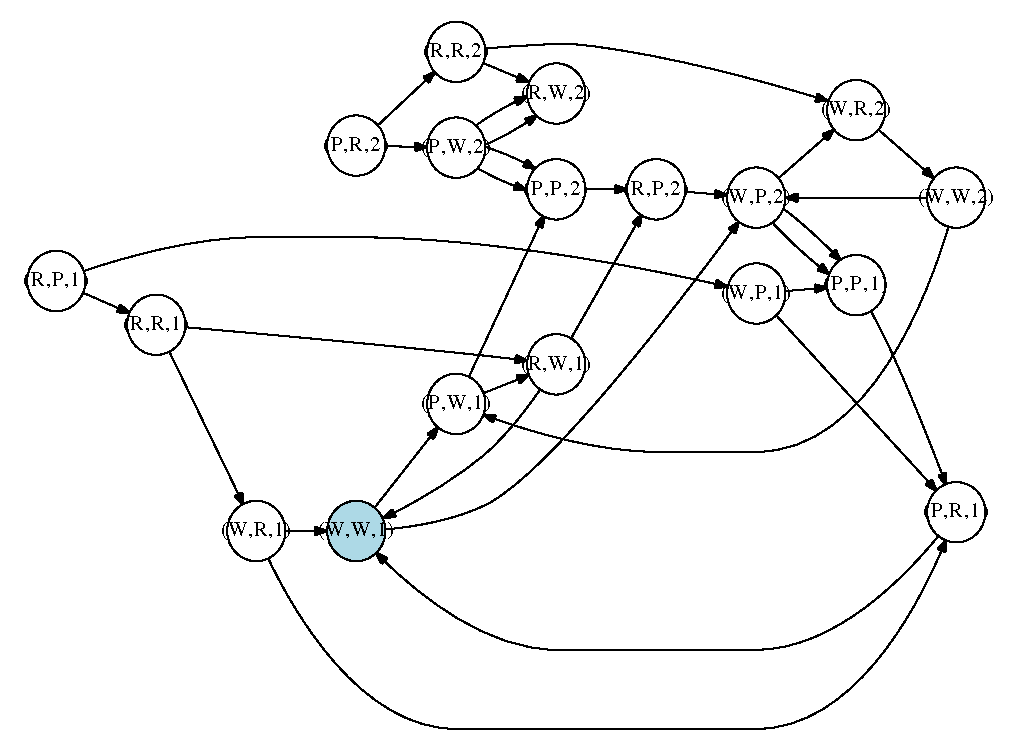
\includegraphics{test.eps}

I don't know why some of them are double lines, they should only be one.
\problempart Adjacency List Representation\\
	Node      -  Adjacency List\\
        "(W,W,1)" - "(P,W,1)", "(W,P,2)";\\

        "(P,W,1)" - "(R,W,1)", "(P,P,2)";\\

        "(R,W,1)" - "(W,W,1)", "(R,P,2)";\\

        "(P,P,2)" - "(R,P,2)";\\

        "(R,P,2)" - "(W,P,2)";\\

        "(W,P,2)" - "(W,R,2)", "(P,P,1)";\\

        "(W,R,2)" - "(W,W,2)";\\

        "(W,W,2)" - "(P,W,1)", "(W,P,2)";\\

        "(W,P,2)" - "(P,P,1)", "(P,R,1)";\\

        "(P,R,1)" - "(W,W,1)";\\

        "(W,P,1)" - "(P,P,1),"(P,R,1)";\\

        "(W,R,1)" - "(P,R,1)", "(W,W,1)";\\

        "(R,P,1)" - "(R,R,1)", "(W,P,1)";\\

        "(R,R,1)" - "(W,R,1)", "(R,W,1)";\\
        
        "(R,R,2)" - "(W,R,2)", "(R,W,2)";\\
        
        "(P,W,2)" -"(P,P,2)", "(R,W,2)";\\
        
        "(P,R,2)" - "(R,R,2)", "(P,W,2)";\\
        
        "(P,W,2)" - "(P,P,2)", "(R,W,2)";\\

\problempart Algorithm to Determine Reachable States\\
Determining the shortest path to all reachable nodes can be done with a modified breath first search.\\
\begin{lstlisting}
initialize distance[] to infinity
init Queue q
enqueue initial node s
distance[s] = 0
while ( q is not empty ):
  u = dequeue()
  print u + d[u] # Outputs Node and length of shortest path to node
  for v in u.adjList():
    if ( distance[v] > d[u] + 1 ):
      enqueue(v)
      d[v] = d[u] + 1
\end{lstlisting}

\problempart Output of Algorithm applied to Peterson's Graph \\
\begin{align*}
WW1 &\; 0\\
PW1 &\; 1\\
WP2 &\; 1\\
RW1 &\; 2\\
PP2 &\; 2\\
WR2 &\; 2\\
PP1 &\; 2\\
RP2 &\; 3\\
WW2 &\; 3\\
PR1 &\; 3\\
\end{align*}
\problempart Safety\\
This proves the safety of the algorithm because none of the reachable states are the forbidden states. Because DFS exhaustively listed all of the reachable states, we know that it is impossible for the algorithm to be unsafe.
\problempart Safety Algorithm without Adjacency List\\
The algorithm above can be modified slightly to determine the safety of the graph only without storing adjacency lists.  \\
The idea is that instead of enqueueing the predetermined adjacency list, use the state transition rules to determine where to go.\\
\begin{lstlisting}
initialize distance[] to infinity
init Queue q
enqueue initial node s
distance[s] = 0
while ( q is not empty ):
  u = dequeue()
  print u + d[u] # Outputs Node and length of shortest path to node
  for v in getListAdjacent(u):
    if ( distance[v] > d[u] + 1 ):
      enqueue(v)
      d[v] = d[u] + 1
      if v = RR1 or RR2:
        return false
return true

def getListAdjacent(Node u):
  # Returns the list of adjacent nodes by applying the rules
\end{lstlisting}

\end{problemparts}

\problem Depth First Lasagna\\
\begin{problemparts}
\problempart Directed Graph\\

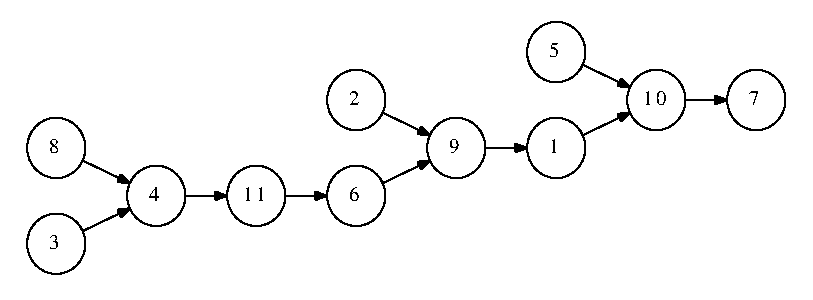
\includegraphics{las.eps}

\problempart Running DFS
The following is a list of the discover and finish events running on the lasgna graph.\\
discover 1\\
discover 10\\
discover 7\\
finish 7\\
finish 10\\
finish 1\\
discover 2\\
discover 9\\
finish 9\\
finish 2\\
discover 3\\
discover 4\\
discover 11\\
discover 6\\
finish 6\\
finish 11\\
finish 4\\
finish 3\\
discover 5\\
finish 5\\
discover 8\\
finish 8\\

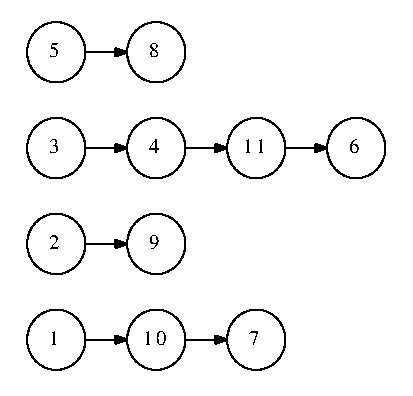
\includegraphics{forest.eps}

I'm not entirely sure on what a DFS forest is supposed to look like.  I made separate trees for each time I exhausted all possible descendants of my source node.\\

\problempart Order of Discover Events\\
The order of discovered events is: 1, 10, 7, 2, 9, 3, 4, 11, 6, 5, 8.  This is not a valid order for multiple reasons, including that it violates the requirement that 4 precede 10.\\

\problempart Using DFS and Topological Sort\\
The reverse order of the finish steps is: 8, 5, 3, 4, 11, 6, 2, 9, 1, 10, 7. This order satisfies all of the constraints.  It also seems like a reasonable order to cook a lasagna.\\

\problempart Why DFS can be used to Topological Sort\\
There is no situation, when performing DFS on a DAG, that there is an edge from u to v, but v finishes after u.\\

It is a property of DFS that all descendants of a node will be processed before the parent node.  So, since there is an edge from u to v, v is a descendent of u.  However, if v did finish after u, then u must be a descendent of v.  The only situation this is possible is if there exists a cycle between the two points, but that is impossible in an acyclic graph, so the described situation never occurs.\\

\problempart DFS for Cyclic Graphs\\
This graph contains a path from u to v, but v appears before u in the DPS tree.\\
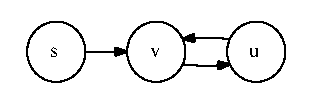
\includegraphics{after.eps}\\
This graph contains a path from u to v, but v appears to the right of u.\\
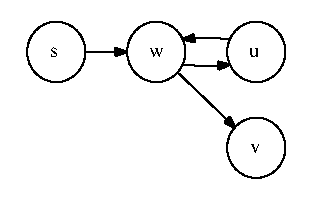
\includegraphics{before.eps}\\
\end{problemparts}
\problem Social Network Structure\\
\begin{problemparts}
\problempart Find Communities\\
To find all communities in a network, I propose to loop through all the vertices, and when encountering one that is not in a community, perform BFS on that node, adding all nodes that are connected to that community. \\
\begin{lstlisting}
init community_hash to all Nones
current_com = 0;
q = empty_queue()
list # This is a list of lists
for all v in V:
  if ( community_hash(v) == None ):
    community_hash(v) = current_com;
    list(current_com) = new list()
    while ( v != null ):
      for u in v.adjacent():
        if ( community_hash(u) == None ):
          community_hash(u) = current_com
          list[current_com].append(v)
          q.euqueue(u)
      v = q.dequeue()

return list
\end{lstlisting}
This algorithm runs in $O(|V| + |E|)$ time.  The outer loop will cycle through all the vertices and do constant work, except when performing BFS, for a time of $O(|V|)$.  That inner loop, which performs the BFS, does a constant amount of work per edge.  While it does revisit nodes, it only vists each edge once, performing $O(|E|)$ work.\\

It is important here to note that, while it might appear to be doing $O(|VE|)$ work, this is not the case.  Consider the two exteme example - the graph is completely connected.  In the outer loop, only the first if check is true, and it traverses all the edges once in the inner loops.  All the other if checks do a constant work unrelated to the number of edges. 
\\

\problempart Conditions Root of DFS Tree is Hub\\
The root of a DFS tree is a hub if it has multiple children.  A property of DFS is that all the descedants are visited before processing the parent. In the DFS tree, this means that all lower levels are processed before the root.  In order for a node to have multiple children, it's right child must not be reachable from any node in the left's subtree.\\

Let's call this potential hub u. If u has only one child, then, because it is a root, it's removal will only disconnect itself from the graph, and it is not a hub.  However, say it has two children, v and w.  Since they are both descedents, and it is an undirected graph, there exists a path (though u) from v to w.  However, v's subtree contains all nodes reachablefrom v without going through u.  Therefore, since w is not in v, the only path from v to w is through u, and u serves as a hub for the community.\\

\problempart Conditions that a Node in a DFS Tree is a Hub\\
If a node, not a root, is a hub, then it holds that there is no descedant of that node that has a back edge to an ancestor of the hub node.  This is true because if such a back edge existed, there would be a path (through that back edge) effectively around the hub node, meaning it wouldn't be a hub. In order for it to be a hub, its removal has to completely separate all nodes below it from the rest of the tree, which only happens in the absense of back edges "over" the hub node.

\problempart Identify Hubs\\
To identify all of the hubs in a graph in $O(|V|+|E|)$ time, first construct the DFS tree, together with the corresponding arrays denoting time visited and time finished, in $O(|V|+|E|)$ time (as in book). Additionally, when constructing this tree, make it doubly linked.\\

Next, traverse the tree backwards (the order DFS finishes nodes) and store, for each node, the most ancestral node it connects to.  There are two possiblities. Either that node has a back edge that links it to a higher (later time finished, earlier visit) node that is higher than all of its children, or, through its children, it is linked to such a node.  This node can be the parent node.\\

When determining this number, you would have to loop through all of a nodes adjacency list to determine the potential backedge node, and then compare that node to its children's highest back edge node, choosing the greater.  In this mannor, after traversal once through the tree (in $O(|V|+|E|)$ time) every node has stored with it the highest node in the tree it can form a path to. \\

Finally, traverse the list of nodes.  If a node has any children whose highest ancestral node is that node, or in other words if there is no path with back edges past the node in question, then that node is a hub.  Another way of saying that is if the most ancestral node that the children of a hub can form a path to is not an ancestor of the hub, then the hub is a real hub.  \\

Additionally, if the node has two or more children, it is a hub automatically.\\

A crucial component of this algorithm is that with the arrays recording time visited and time finished, it is possible to determine, in constant time, whether a node is an ancestor or not.
\end{problemparts}
\end{problems}

\end{document}
